\documentclass[
  11pt,
  letterpaper,
   addpoints,
   answers
  ]{exam}

\usepackage{../exercise-preamble}

\begin{document}

\noindent
\begin{minipage}{0.47\textwidth}

\includegraphics[width=\textwidth]{../fcfm_die}
\end{minipage}
\begin{minipage}{0.53\textwidth}
\begin{center} 
\large\textbf{Conversión de la Energía y Sistemas Eléctricos} (EL4111-1) \\
\large\textbf{Tarea 1} \\
\normalsize Prof.~Constanza Ahumada - Rodrigo Moreno V.\\
\normalsize Prof.~Aux.~Javiera Pacheco - Erik Saez.\\
\normalsize Ayudantes.~Manuel Aceituno - Pamela Acuña - Álvaro Flores 
\end{center}
\end{minipage}

\vspace{0.5cm}
\noindent
\vspace{.85cm}
\hrule
\textbf{Indicaciones: La tarea se puede realizar en grupos de 3 personas. Debe ser entregada el día viernes 13 de septiembre, no se aceptan atrasos, el formato tiene que ser digital (LaTeX, Word, etc.).}
\hrule
\noindent
\vspace{.85cm}
\begin{questions}
    %%%%%%%%%%%%%%%%%%%%%%%%%%%
    \question Considere un cartel de permeabilidad magnética infinita y masa bien distribuida de 0.1 [kg] levitando debajo de un circuito magnético fijo que posee dos núcleos magnéticos semicirculares de iguales dimensiones, con la disposición que se muestra en la figura,tienen radio interno 6 [cm],radio externo 8 [cm] y profundidad de 2 [cm],permeabilidad relativa $\mu_{r} = 2$ para el núcleo asociado a la primera bobina y $\mu_{r} = 3$ para la segunda.
    \begin{figure}[h!]
        \centering
        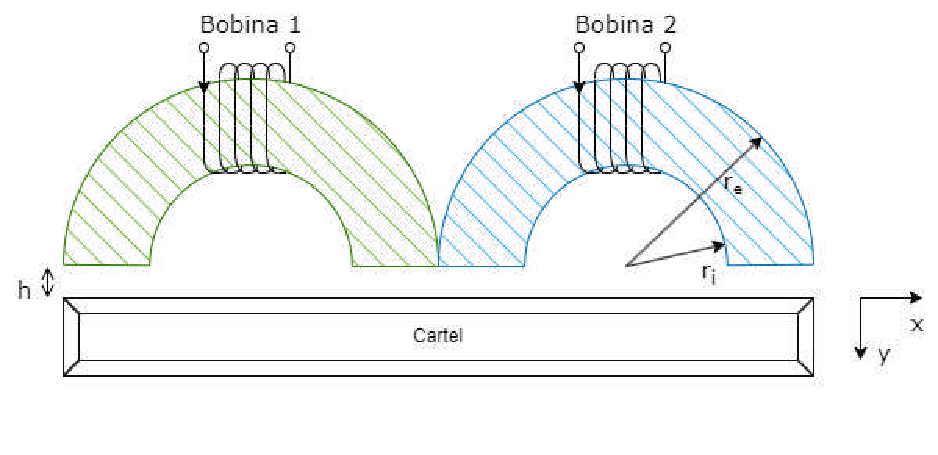
\includegraphics[width=0.5\textwidth]{Tarea_1_1}
    \end{figure}
    \begin{enumerate}[label=\alph*)]
        \item \textbf{(1.5 Puntos)} Calcule el circuito equivalente del sistema,las reluctancias de los elementos presentes y la inductancia propia de cada bobina.
        \item \textbf{(1.5 Puntos)} Encuentre la relación que deben cumplir las fuerzas magnetomotrices para que el cartel no quede desnivelado.
        \item \textbf{(1.5 Puntos)} Considerando que ambas bobinas tienen 200 vueltas,calcule la corriente necesaria en cada bobina para que el cartel quede a 3 [mm] de los núcleos (\textit{Indicación: La fuerza ejercida por un sistema puede calcularse como la derivada de la energía del sistema respecto a la posición h}).
        \item \textbf{(1.5 Puntos)} En un instante dado, se deja de aplicar corriente a la bobina 2,y simultáneamente se aplica una fuerza externa que mueve el cartel hacia arriba y hacia abajo dentro de un rango de h entre 1 [mm] y 5 [mm], siguiendo un movimiento armónico con una frecuencia de 50 [Hz].\textbf{Analice} la fuerza electromotriz (fem) inducida en la segunda bobina. Si existe, calcule su valor en función del tiempo; de lo contrario,justifique su inexistencia.
    \end{enumerate}
    
    %%%%%%%%%%%%%%%%%%%%%%%%%%%

    %%%%%%%%%%%%%%%%%%%%%%%%%%%
    \question Para mantener el voltaje en bornes $v_{0}$ de un generador síncrono,se utiliza un conversor AC/DC como se muestra en la figura.
    \begin{figure}[h!]
        \centering
        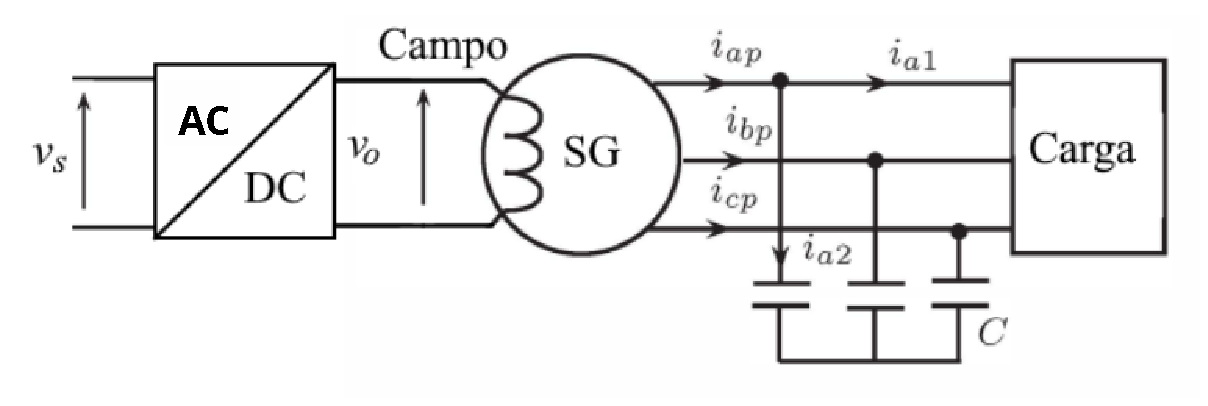
\includegraphics[width=0.5\textwidth]{Tarea_1_2}
    \end{figure}
    \begin{enumerate}[label=\alph*)]
        \item \textbf{(0.5 Puntos)} Considere un rectificador de onda completa y que la frecuencia de la red es de $50$ [Hz] y que su condensador es de $C = 1$ [F],¿Cuál es el valor de $V_{s}$ para poder tener $V_{0} = 120$ [V]?
        \item \textbf{(1 Punto)} Realice el mismo procedimiento y obtenga $V_{s}$ para un rectificador trifásico de onda completa pasivo.¿Cómo cambian sus resultados al usar un rectificador trifásico de onda completa controlado? ¿Cómo influye $\alpha$?
        \item \textbf{(1.5 Puntos)}Simule los tres casos y analice el comportamiento para distintos valores de $C$ y $\alpha$.¿Qué puede concluir con respecto al uso de los 3 rectificadores y los valores de voltaje $V_{s}$ y el tamaño de $C$?\\\\
        Para la realización de la tarea se puede utilizar el software de simulación que estime conveniente (\textit{se recomienda PLECS o MATLAB}).Todos los gráficos deben estar bien rotulados,además mostrar los esquemas realizados en la simulación como los parámetros utilizados.
        \item \textbf{(3 Puntos)} La conexión de paneles solares a la red eléctrica se hace mediante el uso de inversores de potencia.Además,para poder entregar energía cuando la disponibilidad solar es baja se utilizan sistemas de almacenamiento de energía (como baterías de litio). Al respecto, investigue sobre distintas topologías de conexión de paneles solares con sistema de almacenamiento a la red eléctrica (describa al menos 3) y comente sobre las ventajas y desventajas de cada método. Utilice referencias en formato IEEE.
    \end{enumerate}
\end{questions}
\end{document}
